
\documentclass[a4paper,11pt]{article}
\usepackage[utf8]{inputenc}
\usepackage[T1]{fontenc}
\usepackage[frenchb]{babel}

\usepackage{graphicx}
\usepackage{fancyhdr}
\usepackage{geometry}

\usepackage[colorlinks,linkcolor=blue]{hyperref}
\usepackage{amsmath}
\usepackage{amssymb}
\usepackage{mathrsfs}
\usepackage {eurosym}

\usepackage{float}

\geometry{a4paper,tmargin=2cm,bmargin=2cm,lmargin=1.5cm,rmargin=1.5cm,headheight=2.2cm,headsep=0.5cm,footskip=1cm}
\columnsep=0.6cm

\graphicspath{{images/}} 

\usepackage{listings}
\usepackage{color}
\usepackage{xcolor}

\lstset{columns=flexible,keepspaces=true, breaklines,breakindent=0pt} 


\lstset{language=C++,
%basicstyle=\ttfamily,
keywordstyle=\color{blue}\bfseries,
stringstyle=\color{red},
commentstyle=\color{blue!20!black!30!green},
morecomment=[s][\color{black}]{/**}{*/},
numbers=left,
numberstyle=\tiny\color{black},
stepnumber=2,
numbersep=10pt,
tabsize=4,
showspaces=false,
showstringspaces=false}


\fancypagestyle{plain}{
% noms des respo   dans le bas de page                                            
\lfoot{Projet de C++}
\rfoot{M.Morin J.Fourmann}
\renewcommand{\headrulewidth}{0pt}
\fancyhead{}}
% Titre a compl»ter
\title{\textbf{ \huge{Projet de programmation C++}} \\{\Large  Résolution de circuit}}

\author{
\textsc{Jérémie Fourmann} (Promo 2013 - Eléctronique - Enseeiht)\\ %mettre votre nom
\textsc{Maxime Morin} (Promo 2013 - Eléctronique - Enseeiht)\\ %mettre votre nom
%\textsc{ddd dddd} (Promo - departement - respo)     %2 nom
}

\graphicspath{{images/}}

\begin{document}

\pagestyle{plain}

\maketitle
\vspace{1cm}
\renewcommand{\contentsname}{Plan}
\tableofcontents
\vspace{2cm}



\newpage


%Objectif

\section{Objectif}
\section{Organistion du code}
  \subsection{L'objet circuit}
    \begin{figure}[H]
	 \begin{center}
	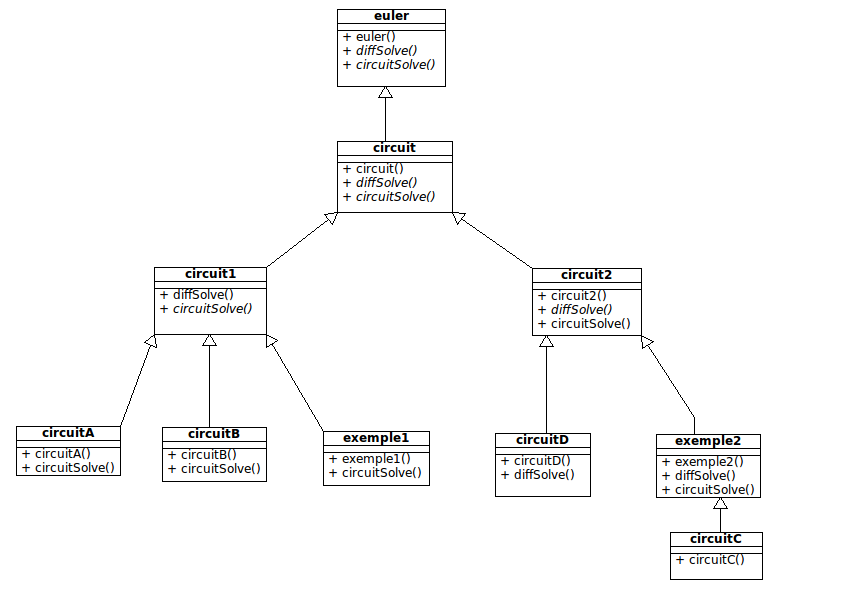
\includegraphics[scale=.7]{circuitDiagram}
	\caption{Hièrarchie de la classe circuit}
	\end{center}
      \end{figure}

  \subsection{L'objet source}
    \begin{figure}[H]
	 \begin{center}
	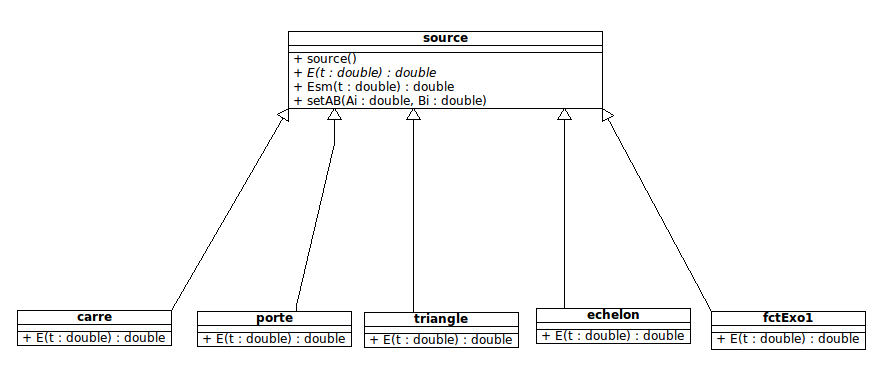
\includegraphics[scale=.7]{sourceDiagram}
	\caption{Hièrarchie de la classe source}
	\end{center}
      \end{figure}
\newpage
\section{Code Source}
  \subsection{main.cpp}
    \lstinputlisting{../main.cpp}
    \newpage
  \subsection{circuits.h}
    \lstinputlisting{../circuits.h}
    \newpage
  \subsection{circuits.cpp}
    \lstinputlisting{../circuits.cpp}
    \newpage
   \subsection{sources.h}
    \lstinputlisting{../sources.h}
    \newpage
   \subsection{sources.cpp}
    \lstinputlisting{../sources.cpp}
    \newpage

\section{Résultats}
  \subsection{Réponse du l'exemple 1}
  \subsection{Réponse du CircuitA}
  \subsection{Réponse du CircuitB}
 
      \begin{figure}[H]
	 \begin{center}
	\includegraphics[scale=1]{C2echelon.pdf}
	\caption{Réponse à un echelon de tension}
	\end{center}
      \end{figure}
      
      \begin{figure}[H]
	      \begin{center}
		\includegraphics[scale=1]{C2porte.pdf}
		\caption{Réponse à une porte}
	      \end{center}
	    \end{figure}

      \begin{figure}[H]
	      \begin{center}
		\includegraphics[scale=1]{C2carre.pdf}
		\caption{Réponse à signal carré}
	      \end{center}
	    \end{figure}

      \begin{figure}[H]
	      \begin{center}
		 \includegraphics[scale=1]{C2triangle.pdf}%fichier généré par -> gnuplot aTrace
		\caption{Réponse à signal triangle}
	      \end{center}
	    \end{figure}
    
  \subsection{Réponse du CircuitC}
  \subsection{Réponse du CircuitD}
\end{document}
